\chapter{综合分析}
本设计采用固溶-时效工艺对合金进行处理。

固溶处理的目的是为了使合金在高温状态下内部合金元素发生充分扩散,促使 一定体积分数的 α→β 转变,然后在较快冷却条件下抑制连续冷却过程中 β→α 转变, 从而获得 α′相、α′′相以及 β′相等亚稳定相,为后期的时效处理提供良好的组织状态。 时效处理的目的是通过将固溶处理过程中得到的亚稳定相加热到一定温度进行等温 处理,在热力学的条件下,促使亚稳定相向稳定状态转变,产生细小弥散分布的析 出相,从而对钛合金起到强化作用。

TC4 钛合金在稳定状态下含有少量的 β 相,β 相的存在使其具有热处理强化的能 力。由\ref{fig:tc4change}可知,固溶处理过程中固溶温度对固溶后的亚稳定相种类起决定作 用,不同固溶温度下 α 与 β 相的平衡体积分数不同,造成 β 相中合金元素含量不同, 从而在快速冷却过程中产生不同的亚稳定相。
\begin{figure}[h!]
	\centering
	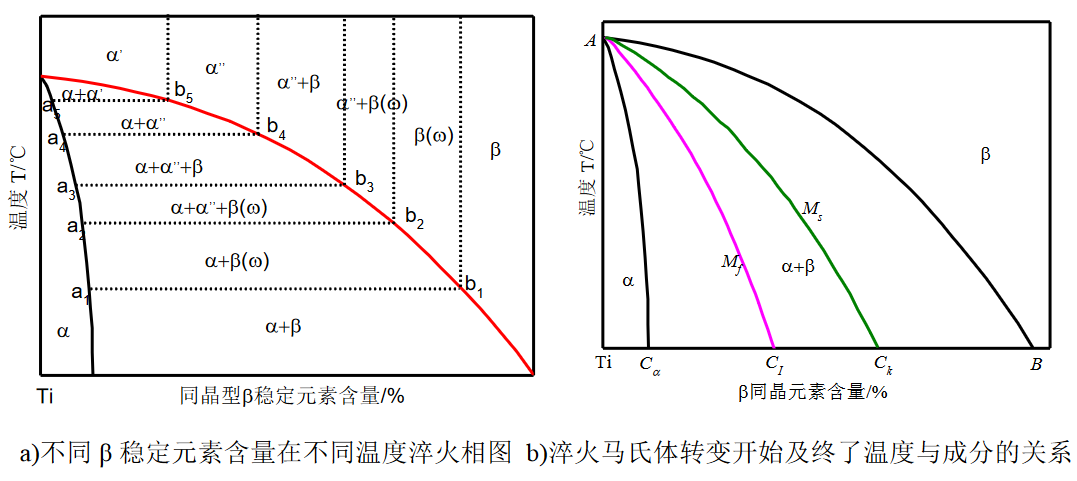
\includegraphics[width=0.7\linewidth]{pic/tc4change}
	\caption{钛合金在淬火过程中的亚稳定相及马氏体转变温度}
	\label{fig:tc4change}
\end{figure}
\section{固溶处理的影响}
\subsection{固溶温度对组织性能的影响}
钛合金在进行固溶处理时,固溶温度对其在高温平衡状态下 α 相体积分数具有 决定性作用。
选取经 910°C、950°C与 990°C分别固溶 1h 水冷的显微 组织进行观察,如所示。可以看出在 α+β 两相区进行固溶后水冷,显微组织 为初生的等轴 α 相与细针 α′状马氏体组成;由图 3-4 e)所示,在 β 单相区进行固溶后 水冷,显微组织为粗大的原始 β 晶粒内部分布着单一的细针状马氏体,马氏体在晶 内交错排列,夹角成 60 度或 90 度。

\begin{figure}[h!]
	\centering
	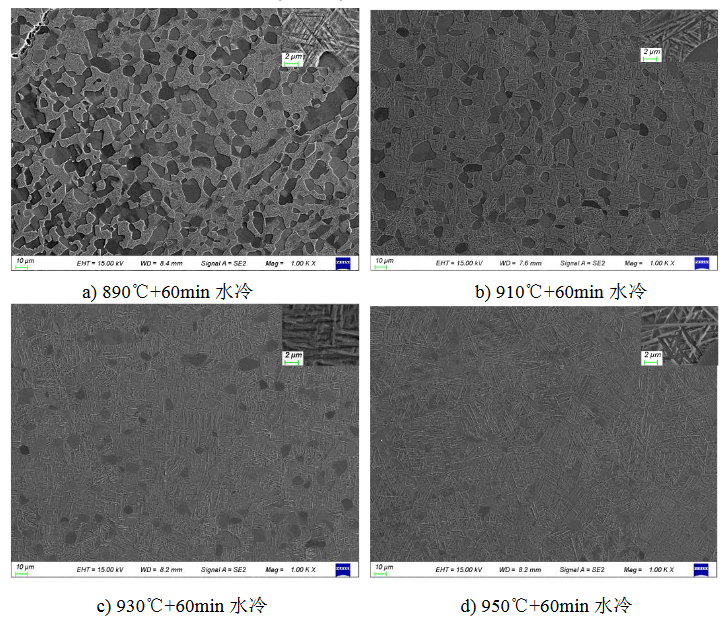
\includegraphics[width=0.7\linewidth]{pic/demo-不同固溶温度的影响}
	\caption{不同固溶温度下的组织}
	\label{fig:demo-}
\end{figure}


\subsection{冷却方式对组织性能的影响}
图 3-2 为 TC4 钛合金经 950°C保温 1 小时分别进行油冷和水冷后的显微组织形 貌,从图中可以看出,油冷后组织主要是由初生等轴 α 相和 β 转变组织组成的双态 组织,水冷后组织主要是由等轴初生 α 相和针状马氏体组成。TC4 钛合金在加热过 程中,随着温度的升高,α 相逐渐转变为 β 相,当加热温度未高于相变点温度时,高 温状态下组织由未溶解的初生等轴 α 相和 β 相构成。在连续冷却过程中,未溶解的 初生等轴 α 相进行扩散型长大,由于油冷的冷却速率小于水冷,初生等轴 α 相的长 大时间要多于水冷,造成油冷后初生等轴 α 相的晶粒尺寸大于水冷。利用 XRD 分析 了固溶后经不同冷却方式后的相组成,如图 3-3 所示。

\begin{figure}[h!]
	\centering
	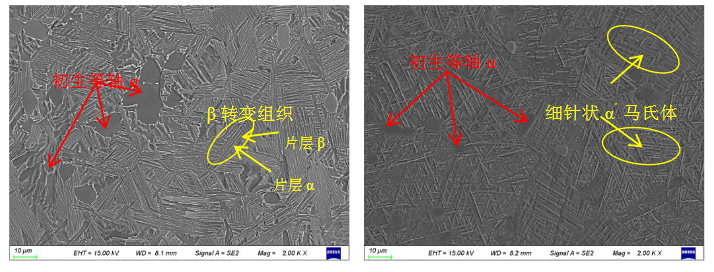
\includegraphics[width=0.7\linewidth]{pic/demo-油冷与水冷的对比}
	\caption{不同冷却方式下的 TC4 钛合金显微组织}
	\label{fig:demo-油冷与水冷}
\end{figure}

TC4 钛合金 950°C固溶分别经油冷和 水冷后,相的组成存在较大差异,油冷时的冷却速率较低,高温 β 相中的合金元素 在冷却过程中发生扩散,进行扩散型相变,导致次生 α 相在初生 α 与 β 相界面处形 核,并向 β 相晶内长大,生成 α 片层与 β 片层相间的 β 转变组织,最终相的构成包 α 相与 β 相;水冷时的冷却速率极快,冷却过程基本在瞬间完成,导致 β→α 的扩散型 相变来不及发生,β 相通过晶格切变的形式进行原子集体的、有规律的近程迁移,生 成 α′马氏体,最终相的构成包含 α 相与 α′相,没有发现 β 相存在。


\section{时效处理的影响}
\subsection{时效温度对组织性能的影响}

时效处理时组织转变的物质基础是:固溶或者退火处理得到的马氏体$ \alpha^{\prime} $相和亚稳$ \beta $相,这两种相是热力学上不稳定的物质,加热时会分解。

固溶在高温下将大量的 $\alpha$ 相转变 为 $\beta$ 相, 然后进行快速冷却, 可以防止过多的 $\beta$ 相 转变为 $\alpha$ 相。在保留了高温 $\beta$ 组织的同时, 发生了马氏体相变,部分 $\beta$ 相转变为不稳定的 $\alpha^{\prime}$ 相和 $\alpha^{\prime \prime}$ 相, 为时效相转变提供了良好的组织\cite{ xinsheweiGuanyutaihejinrechulihexichuxiangdetaolun2006,zouhaibeiTC4taihejinrechuliqianghuagongyijixiangbianhangweiyanjiu2019a}。时效处理通过对亚稳定组织低温热处理, 促使亚稳定组织 $\beta$ 相、$ \alpha  ^{\prime}$相及 $ \alpha  ^{\prime\prime}$相转变为细小、室温稳定的等轴组织与片层组织,以起到弥散强化作用,改善组织的塑性和韧性。常见的组织为\cite{zhanghaoyinGurongShixiaoduiTC4taihejinzuzhihelixuexingnengdeyingxiang2014}: $ \alpha  ^{\prime}$相、$ \alpha  ^{\prime}$相脱溶出来的等轴$ \alpha$相与$ \beta $相、变粗大的$ \alpha $相、 $ \beta $相。

对于固溶-时效组合处理工艺而言,固溶后TC4钛合金中马氏体仍保持$ \alpha $相软而韧的性能,在随后进行时效强化可以使得马氏体分解,获 得 弥 散 的轴$ \alpha+\beta $组织,从而进一步提高其抗拉强度。 但随 着 时 效 温度的升高,伸长率会逐 渐 上 升,抗拉强度则呈下降趋势。当时效温度过高时,组织会粗化,使合金的塑性、韧性下降\cite{guxiaohuiCuihuoShixiaowenduduiTC4taihejinzuzhihelixuexingnengdeyingxiang2011}。

时效处理温度主要影响\ti 合金中次生$ \alpha $的尺寸,Sauer\cite{sauerThermomechanicalProcessingHigh2001}等人研究发现\ti 合金中沿着$ \beta $晶界形成的连续$ \alpha  $片层组织对合金的机械加工性能有负面影响,等轴$ \beta $相越大,负面作用越强烈;经过重结晶等匀质化处理后,可以调整$ \alpha $相的体积分数,进而改善性能。鲁媛媛、马保飞\cite{luyuanyuanShixiaochuliduiTC4taihejinweiguanzuzhihelixuexingnengdeyingxiang2019}等人研究了970℃固溶处理之后,在不同固溶温度下合金的组织,研究发现,当时效温度在 $450{ }^{\circ} \mathrm{C}$ 到 $550{ }^{\circ} \mathrm{C}$之间时 ,随温度增加,合金的强度值 逐渐增加; 但当温度大于 $600{ }^{\circ} \mathrm{C}$ 时,强度随温度增加而逐渐下降,当时效温度为 $550{ }^{\circ} \mathrm{C}$ 时,合金的强度最高。李露\cite{lilouGurongshixiaoduiTC4hejinzuzhiyujixiexingnengdeyingxiang2014}研究发现TC4合金的硬度随时效温度的升高而下降,当 固溶快冷组织为亚稳 的 $\beta 、 \alpha^{\prime} 、 \alpha^{\prime\prime}$ 相,时 时效过程分解产物为弥散的 $\alpha$ 和 $\beta$ 相, 而且时效温度越高, 分解越充分, 硬度越低。

顾晓辉\cite{guxiaohuiCuihuoShixiaowenduduiTC4taihejinzuzhihelixuexingnengdeyingxiang2011}人研究发现同等条件下,时效温度越低,$ \alpha^{\prime} $转变得到的$ \alpha+\beta  $相组织越细小,越弥散;当固溶温度提高时,组织变粗,这与二次$ \beta $相的分解密切相关,当初生$ \alpha $相的尺寸较大时,随时效温度升高,析出的$ \alpha $相会与初生$ \alpha $相聚集长大,发生球化。

在时效后的得到等轴组织和双态组织中,均含有一定量的等轴初 生 $\alpha$ 相。而拉伸变形通常是在等轴初生 $\alpha$ 相的某晶粒开始滑移,裂纹往往在在相界面上产生。 变形过程中,随着变形量的增大, 初生$\alpha$ 晶粒会产生更多的滑移, 并 向周围的 $\beta$ 转变组织扩展, 导致空洞形核、和扩展变慢迟, 断裂前将产生更大的变形, 从而获更高的塑性\cite{yekangyuanRechuliduiTC4taihejinduanjianzuzhihexingnengdeyingxiang2022}。

\section{结论}
